\newcommand{\svcourse}{CST Part IA: Software Engineering and Security}
\newcommand{\svnumber}{1}
\newcommand{\svvenue}{Microsoft Teams}
\newcommand{\svdate}{2022-05-11}
\newcommand{\svtime}{15:00}
\newcommand{\svuploadkey}{CBd13xmL7PC1zqhNIoLdTiYUBnxZhzRAtJxv/ytRdM1r7qIfwMsxeVwM/pPcIo8l}

\newcommand{\svrname}{Dr Sam Ainsworth}
\newcommand{\jkfside}{oneside}
\newcommand{\jkfhanded}{yes}

\newcommand{\studentname}{Harry Langford}
\newcommand{\studentemail}{hjel2@cam.ac.uk}


\documentclass[10pt,\jkfside,a4paper]{article}

% DO NOT add \usepackage commands here.  Place any custom commands
% into your SV work files.  Anything in the template directory is
% likely to be overwritten!

\usepackage{fancyhdr}

\usepackage{lastpage}       % ``n of m'' page numbering
\usepackage{lscape}         % Makes landscape easier

\usepackage{verbatim}       % Verbatim blocks
\usepackage{listings}       % Source code listings
\usepackage{graphicx}
\usepackage{float}
\usepackage{epsfig}         % Embed encapsulated postscript
\usepackage{array}          % Array environment
\usepackage{qrcode}         % QR codes
\usepackage{enumitem}       % Required by Tom Johnson's exam question header

\usepackage{hhline}         % Horizontal lines in tables
\usepackage{siunitx}        % Correct spacing of units
\usepackage{amsmath}        % American Mathematical Society
\usepackage{amssymb}        % Maths symbols
\usepackage{amsthm}         % Theorems

\usepackage{ifthen}         % Conditional processing in tex

\usepackage[top=3cm,
            bottom=3cm,
            inner=2cm,
            outer=5cm]{geometry}

% PDF metadata + URL formatting
\usepackage[
            pdfauthor={\studentname},
            pdftitle={\svcourse, SV \svnumber},
            pdfsubject={},
            pdfkeywords={9d2547b00aba40b58fa0378774f72ee6},
            pdfproducer={},
            pdfcreator={},
            hidelinks]{hyperref}

\renewcommand{\headrulewidth}{0.4pt}
\renewcommand{\footrulewidth}{0.4pt}
\fancyheadoffset[LO,LE,RO,RE]{0pt}
\fancyfootoffset[LO,LE,RO,RE]{0pt}
\pagestyle{fancy}
\fancyhead{}
\fancyhead[LO,RE]{{\bfseries \studentname}\\\studentemail}
\fancyhead[RO,LE]{{\bfseries \svcourse, SV~\svnumber}\\\svdate\ \svtime, \svvenue}
\fancyfoot{}
\fancyfoot[LO,RE]{For: \svrname}
\fancyfoot[RO,LE]{\today\hspace{1cm}\thepage\ / \pageref{LastPage}}
\fancyfoot[C]{\qrcode[height=0.8cm]{\svuploadkey}}
\setlength{\headheight}{22.55pt}


\ifthenelse{\equal{\jkfside}{oneside}}{

 \ifthenelse{\equal{\jkfhanded}{left}}{
  % 1. Left-handed marker, one-sided printing or e-marking, use oneside and...
  \evensidemargin=\oddsidemargin
  \oddsidemargin=73pt
  \setlength{\marginparwidth}{111pt}
  \setlength{\marginparsep}{-\marginparsep}
  \addtolength{\marginparsep}{-\textwidth}
  \addtolength{\marginparsep}{-\marginparwidth}
 }{
  % 2. Right-handed marker, one-sided printing or e-marking, use oneside.
  \setlength{\marginparwidth}{111pt}
 }

}{
 % 3. Alternating margins, two-sided printing, use twoside.
}


\setlength{\parindent}{0em}
\addtolength{\parskip}{1ex}

% Exam question headings, labels and sensible layout (courtesy of Tom Johnson)
\setlist{parsep=\parskip, listparindent=\parindent}
\newcommand{\examhead}[3]{\section{#1 Paper #2 Question #3}}
\newenvironment{examquestion}[3]{
\examhead{#1}{#2}{#3}\setlist[enumerate, 1]{label=(\alph*)}\setlist[enumerate, 2]{label=(\roman*)}
\marginpar{\href{https://www.cl.cam.ac.uk/teaching/exams/pastpapers/y#1p#2q#3.pdf}{\qrcode{https://www.cl.cam.ac.uk/teaching/exams/pastpapers/y#1p#2q#3.pdf}}}
\marginpar{\footnotesize \href{https://www.cl.cam.ac.uk/teaching/exams/pastpapers/y#1p#2q#3.pdf}{https://www.cl.cam.ac.uk/\\teaching/exams/pastpapers/\\y#1p#2q#3.pdf}}
}{}


\usepackage[T1]{fontenc}
\lstset{upquote=true}
\usepackage{tikz}

\begin{document}

\section{Introduction to Genetics}

\begin{enumerate}

    \item Describe the structure of the \textit{deoxyribonucleic acid} (DNA), and highlight the ways in which it differs from the \textit{ribonucleic acid} (RNA). Distinguish the concepts of a gene and a genome
    with respect to DNA structure.

    DNA is a double helix structure: it consists of two sequences of bases (abbreviated \texttt{ATCG}) which are bound together in complimentary pairs: \texttt{A} binds with \texttt{T}; and \texttt{C} binds
    with \texttt{G}. A gene is a sequence of DNA which represents a protein which perform a particular function. The genome is the entirety of all the DNA in an organism. This consists of a set of chromosomes
    -- each of which is composed of thousands of genes.

    Rather than having the bases \texttt{ATCG}, RNA has the bases \texttt{AUCG} where \texttt{A} binds with \texttt{U}. In the context of eukaryotic cells, DNA is found in the nucleus while RNA is found around
    the cell. There are 3 types of RNA\@. The most important of which is mRNA; which is read by ribosomes and used to guide them which proteins to synthesise.

    \item Explain, with the aid of a diagram, the process of \textit{gene expression} (synthesis of a protein based on the genetic information contained within DNA). Your answer should contain the following terms:

    \begin{itemize}

        \item DNA

        \item messenger RNA

        \item codon

        \item protein

        \item transcription

        \item translation

    \end{itemize}

    We have DNA in the nucleus. It's transcribed into mRNA by RNA polymerase enzymes. This mRNA then leaves the nucleus. It is then found by some ribosomes. They then inspect the codons (sequences of 3 bases)
    and translate this into the corresponding proteins.

    \item How are different genes delimited within the DNA molecule? Can you correlate this to a similar concept used within a programming language (covered within the Tripos)?

    Genes are preceded by a regulatory region. They have buffer space at the end to reduce the probability that during transcription, ribosomes will overread the gene and read into another gene. This is related
    to the memory representation of arrays in languages such as \texttt{C} when running with ASan. Arrays are started by a pointer and terminated by a null pointer. Furthermore, at the end of each array there is
    a set of uninitialised memory to act as a buffer to reduce the risk of accidental overflow.

    \item How many different codons exist? How about different amino acids? Provide an \textit{evolutionary} explanation for the discrepancy between your two answers.

    There are 64 different codons ($4^3$). There are 20 amino acids which are represented by codons (plus STOP). This gives redundancy and tries to reduce the probability that a protein will be badly
    mis-synthesised. Furthermore, most of the redundancy is in the third base in the codon: this is because the third base is the most likely to mutate. This happened because those animals which had fewer amino
    acids were less likely to suffer from frequent mis-synthesis and so their bodies worked better and they ended up with a higher survival rate.

\end{enumerate}

\section{Sequence Alignment}

\begin{enumerate}

    \item Describe in detail the dynamic programming algorithm used for computing a \textit{global alignment} between two DNA sequences, noting its inputs, outputs and time complexity. Explain the significance
    of the \textit{score matrix} in this context, and provide a score matrix that would convert this problem into the familiar LCS (\textit{longest common subsequence}) problem.

    \begin{definition}[Score Matrix]

        A score matrix $S$ is a similarity matrix where the element $S_{i, j}$ indicates how similar the $i^{\text{th}}$ symbol is to the $j^{\text{th}}$ symbol. This allows us to model similarity between codon
        and represent that dissimilar mutations are unlikely, leading to substantially better approximations with no additional complexity.

    \end{definition}

    \begin{question}[Symmetry of Score Matrices]

        Is there ever a situation where we would want a score matrix that is \textit{not} symmetric? Why would this be useful?

    \end{question}

    \begin{definition}[Needleman-W\"unsch algorithm]

        The simplest possible algorithm to solve the Global Alignment problem. It takes as input two strings $v, w \in \Sigma^*$ and a score matrix $S$ for the language $\Sigma \cup \{\_\}$ and provides as an
        output an alignment of $v$ and $w$ whose alignment score is maximal.

    \end{definition}

    \begin{lstlisting}[language=python, mathescape=true]

def needleman_wunsch(v: str, w: str, S: dict[tuple[str, str], float]):
    mem = [[None for _ in range(len(w))] for _ in range(len(v))]
    mem[0, 0] = 0
    ptr = [[None for _ in range(len(w))] for _ in range(len(v))]
    mem[0, 0] = "$\bullet$"

    for i in range(1, len(v)):
        mem[i, 0] = mem[i - 1, 0] - S["_", v[i - 1]]
        ptr[i, 0] = "$\uparrow$"

    for j in range(1, len(w)):
        mem[0, j] = mem[0, j - 1] - S["_", w[j - 1]]
        ptr[0, j] = "$\leftarrow$"

    for i in range(1, len(v) + 1):
        for j in range(1, len(w) + 1):
            mem[i][j] = max(
                mem[i - 1][j - 1] + score[v[i - 1], w[j - 1]],
                mem[i - 1][j] + score["_", w[j - 1]],
                mem[i][j - 1] + score["_", v[i - 1]],
            )
            match mem[i][j]:
                case mem[i - 1][j - 1] + S[v[i], w[j]]:
                    ptr[i][j] = "$\nwarrow$"
                case mem[i - 1][j] - S[\_, v[i - 1]]:
                    ptr[i][j] = "$\uparrow$"
                case mem[i][j - 1] - S[\_, w[j - 1]]:
                    ptr[i][j] = "$\leftarrow$"

    return mem, ptr

    \end{lstlisting}

    A matrix which would convert this problem into LCS is given below:
    \[
        \begin{pmatrix}
            1 & -\infty & \cdots & -\infty& 0 \\
            -\infty& 1 & \cdots & -\infty& 0 \\
            -\infty& -\infty& \cdots & -\infty& 0 \\
            \vdots & \vdots & \vdots & \vdots & \vdots \\
            -\infty& -\infty& \cdots & 1 & 0 \\
            0 & 0 & \cdots & 0 & 0 \\
        \end{pmatrix}
    \]

    \item Implement your algorithm from question 1 in a language of your choice and use it to compute the global alignment (and alignment score) of the sequences \texttt{CGTGAA} and \texttt{GACTTAC}, with the
    following parameters:

    \begin{itemize}

        \item Match: $+5$

        \item Mismatch: $-3$

        \item Insertion / deletion: $-4$

    \end{itemize}

    You may also verify your result by computing it manually -- it is good practice for the examinations.

    My implementation computed that the maximum alignment between the two strings according to the score matrix given is $-3$. This is validated by manually carrying out the computation.

    \begin{table}[h]

        \centering

        \begin{tabular}{c|ccccccccccccc}
            && \texttt{C} && \texttt{G} && \texttt{T} && \texttt{G} && \texttt{A} && \texttt{A} & \\
            \hline
            & $0$ && $-4$ && $-8$ && $-12$ && $-16$ && $-20$ && $-24$ \\
            \texttt{G} &&&&&&&&&&&&&\\
            & $-4$ && $-3$ && $1$ && $-3$ && $-7$ && $-11$ && $-14$ \\
            \texttt{A} &&&&&&&&&&&&&\\
            & $-8$ && $-7$ && $-6$ && $-2$ && $-6$ && $-2$ && $-6$ \\
            \texttt{C} &&&&&&&&&&&&&\\
            & $-12$ && $-3$ && $-7$ && $-7$ && $-5$ && $-6$ && $-5$ \\
            \texttt{T} &&&&&&&&&&&&&\\
            & $-16$ && $-7$ && $-6$ && $-2$ && $-6$ && $-9$ && $-9$ \\
            \texttt{T} &&&&&&&&&&&&&\\
            & $-20$ && $-11$ && $-10$ && $-1$ && $-5$ && $-9$ && $-12$ \\
            \texttt{A} &&&&&&&&&&&&&\\
            & $-24$ && $-15$ && $-14$ && $-5$ && $-4$ && $0$ && $-4$ \\
            \texttt{C} &&&&&&&&&&&&&\\
            & $-28$ && $-19$ && $-18$ && $-9$ && $-8$ && $-4$ && $-3$ \\
        \end{tabular}

    \end{table}

    \item Outline the key transformations that need to be made to the algorithm in order to find optimal \textit{local alignments}, as well as incorporating \textit{affine gap penalties}. why are these features
    useful? Have you changed the time complexity of the algorithm by doing so?

    \begin{definition}[Local Alignment Problem]

        In the Local Alignment Problem, we take two strings $v$ and $w$ as input, and a score matrix. The output is then substrings $s_v$, $s_w$ of $v$, $w$ such that the global alignment between $s_v$ and $s_w$
        is maximised.

    \end{definition}

    We can augment the Needleman-W\"unsch Algorithm by initialising the edges of the graph to $0$. This has the effect of ignoring the cost of any regions at the start or end of strings with low alignment. This is
    now the Smith-Waterman Algorithm for solving the Local Alignment Problem. This has both the same time and space complexity as the Needleman-W\"unsch Algorithm.

    \begin{definition}[Affine Gaps Problem]

        In the Affine Gaps Problem, we model the cost of a gap as of length $g$ as $d + e \times (g - 1)$. The reasoning behind this is that larger gaps are probably caused by the same event and so should not be
        penalised as heavily. The input is two strings $u$, $v$ and a score matrix. The output is an Alignment which has a minimal cost assuming we use Affine Gap Penalties.

    \end{definition}

    There are two algorithms given for the Affine Gaps problem. One is an exact solution and the second is an inexact solution which the paper which Pietro extracted it from claims that it has small impact in
    most cases: and is correct in the case where $-d - e < \min(S)$. I provide the augmentations required to implement both.

    In the exact solution, we have three matrices: \texttt{lower} stores the best cost alignment that ends in insertions; the best overall alignment; and the best alignment which ends in deletions. The exact
    algorithm is implemented by the following algorithm:

    \begin{lstlisting}[language=python]

def affine_gaps(v: str, w: str, score, e, d):
    lower = [[None for _ in range(len(w) + 1] for _ in range(len(w) + 1)]
    middle = [[None for _ in range(len(w) + 1] for _ in range(len(w) + 1)]
    upper = [[None for _ in range(len(w) + 1] for _ in range(len(w) + 1)]

    lower[0][0] = -e
    middle[0][0] = 0
    upper[0][0] = -e

    for i in range(1, len(v) + 1):
        lower[i][0] = -e - d * (i - 1)
        middle[i][0] = -e - d * (i - 1)

    for j in range(1, len(w) + 1):
        middle[0][j] = -e - d * (i - 1)
        upper[0][j] = -e - d * (i - 1)

    for i in range(1, len(v) + 1):
        for j in range(1, len(w) + 1):
            lower[i][j] = max(
                lower[i - 1][j] - d,
                middle[i - 1][j] - e,
            )
            upper[i][j] = max(
                upper[i][j - 1] - d,
                middle[i][j - 1] - e,
            )
            middle[i][j] = max(
                lower[i][j],
                upper[i][j],
                middle[i - 1][j - 1] + S[v[i - 1], w[j - 1]]
            )

    return middle[-1][-1]

    \end{lstlisting}

    The second algorithm gets an inexact solution. It only uses two matrices. The first \texttt{F} stores the optimal alignment; and the second \texttt{G} stores the optimal alignment which ends in a gap. The
    problem with this algorithm is that we consider a gap in one string followed by a gap in the \textit{other} as a single gap and thus provide the affine penalty when creating it. The justification for this
    algorithm is that it only inexact in regions which have bad alignment anyway. I don't understand why this justifies a broken algorithm.

    \begin{lstlisting}[language=python]

def affine_gaps(v: str, w: str, score, e, d):
    F = [[None for _ in range(len(w) + 1)] for _ in range(len(v) + 1)]
    G = [[None for _ in range(len(w) + 1)] for _ in range(len(v) + 1)]

    F[0][0] = 0
    G[0][0] = 0

    for i in range(1, len(v) + 1):
        F[i][0] = -e - d * (i - 1)
        G[i][0] = -e - d * (i - 1)

    for j in range(1, len(w) + 1):
        F[0][j] = -e - d * (i - 1)
        G[0][j] = -e - d * (i - 1)

    for i in range(1, len(v) + 1):
        for j in range(1, len(w) + 1):
            G[i][j] = max(
                G[i - 1][j] - d,
                G[i][j - 1] - d,
                F[i - 1][j] - e,
                F[i][j - 1] - e,
            )
            F[i][j] = max(
                G[i][j],
                F[i - 1][j - 1] + S[v[i - 1], w[j - 1]]
            )

    return F[-1][-1]

    \end{lstlisting}

    \item Provide an explanation (accompanied with a brief pseudocode and diagram) of how the storage complexity of the global alignment algorithm can be significantly reduced, while keeping time complexity the
    same. Provide an informal proof that the asymptotic time complexity does not increase.

    In the main iteration step, when we fill in the table, the current row only ever depends on the previous row. This means we can find the minimum cost alignment using only two rows: we deallocate the previous
    row when we have finished computing the next one since we will never use it again! However, this algorithm only computes the cost of the optimum global alignment.

    To get the alignment as well as its cost, note that we can simultaneously both work forwards to the middle of the string and backwards from the end of the string. When these two algorithms meet in the middle
    at index \texttt{mid} of the first string, we have two columns: \texttt{prefix} and \texttt{suffix}, where \texttt{prefix}[\texttt{i}] is ``the greatest alignment between $v[:\texttt{mid}]$ and
    $w[:\texttt{i}]$''; and \texttt{suffix}[\texttt{i}] is ``the greatest alignment between $v[\texttt{mid}:]$ and $w[\texttt{i}:]$''. So notice that $\texttt{length}[\texttt{i}]\texttt{prefix}[\texttt{i}] +
    \texttt{suffix}[[\texttt{i}]]$ is the cost of the best alignment which passes through the vertex $[\texttt{mid}, \texttt{i}]$. We can then divide the size of the problem in half and solve each case
    recursively. If we resolve duplicates consistently, then we can compute the optimal alignment in quadratic time and polynomial space. Essentially, we compute a node in the middle of the alignment in
    quadratic time and linear space. However, since we halve the size of the problem each time, the complexity is still quadratic.

    \[
        T(n) = n^2 + 2 \cdot T\left( \frac{n}{2} \right) \implies T(n) = 2 \cdot n^2 \in \mathcal O\left( n^2 \right)
    \]

    A strange algorithm where you only compute half of the nodes and instead run an algorithm to compute the successor. This doesn't decrease the real time or the complexity. Furthermore, it doesn't make sense
    since we can easily compute the predecessor as well, which would reduce the number of nodes we have to compute by the exact same amount! Thus this optimisation appears not to give any advantage: and even if
    it did it would only be exploiting half the potential for optimisation.

    I provide a working python implementation in the next question so shall not provide pseudocode

    \item Implement the reduced storage variant of the global alignment algorithm in a language of your choice, and verify that it provides the same result for the inputs in question 2.

    \lstinputlisting[language=python]{reduced_storage.py}

    \item Describe the Nussinov algorithm for RNA secondary structure prediction, its underlying assumptions and time/storage complexities. What should be the output of the algorithm on the sequence
    \texttt{GCAACGUCG}? (this is a test of understanding -- do not actually perform the algorthm on this sequence!)

    \begin{definition}[Nussinov Algorithm]

        A dynamic programming algorithm for predicting how RNA will fold. It starts by considering the most likely substructures of length 1, then iteratively uses the most likely substructures of length $i$ to
        compute the most likely substructures of length $i + 1$. Nussinov's algorithm can model bulges, internal loops and multiloops. However, a critical limitation is that it \textit{cannot model pseudoknots}!
        This makes it an oversimplification that is not used in practice.

    \end{definition}

    Nussinov's algorithm has a space complexity of $\mathcal O(n^2)$ for a sequence of length $n$ and a time complexity of $\mathcal O(n^3)$. The additional time complexity comes from looking back for potential
    substructures which may merge (\ie allowing substructures other tha a single stem with bulges and internal loops).

    In the example given, the algorithm would output that \texttt{C} binds with \texttt{G}, \texttt{A} with \texttt{U} and \texttt{C} with \texttt{G}.

    \begin{figure}[H]

        \centering

        \begin{tikzpicture}

            \node (1) at (1, 0) {$G$};
            \node (2) at (1, 1) {$C$};
            \node (3) at (0, 2) {$A$};
            \node (4) at (1, 3) {$A$};
            \node (5) at (1, 4) {$C$};
            \node (6) at (2, 4) {$G$};
            \node (7) at (2, 3) {$U$};
            \node (8) at (3, 2) {$G$};
            \node (9) at (2, 1) {$G$};

            \path (1) edge (2);
            \path [bend left] (2) edge (3);
            \path [bend left] (3) edge (4);
            \path (4) edge (5);
            \path [bend left] (5) edge (6);
            \path (6) edge (7);
            \path [bend left] (7) edge (8);
            \path [bend left] (8) edge (9);

            \draw [dashed] (2) -- (9);
            \draw [dashed] (4) -- (7);
            \draw [dashed] (5) -- (6);

        \end{tikzpicture}

        \caption{A diagram of a possible folding for the sequence \texttt{GCAACGUCG}}

    \end{figure}

\end{enumerate}

\section{Phylogeny}

\begin{enumerate}

    \item Compare and contrast the \textit{distance-based} with \textit{parsimony-based} approaches to constructing phylogenetic trees, and comment on their relative merits.

    I consider the distance-based approaches to phylogeny to be UPGMA and Neighbour Joining; while the parsimony based approaches are the algorithms which solve the small/large parsimony problems.

    Distance-based approaches to phylogeny are more resistant than parsimony based approaches: parsimony based approaches do not allow comparisons between strings which do not have the same length. Furthermore,
    parsimony-based approaches can have strings which are very similar to each other rated very differently: they suffer from the problem with hamming distances (\ie that they do not take account of insertion or
    deletion thus \texttt{TATATATAT} and \texttt{ATATATATA} would be rated very differently).

    The large parsimony is an NP-complete problem doesn't have an exact solution: this means that the algorithms that solve it are not exact and have no guarantees. No good polynomial-time approximation
    algorithm exists for problems like this. The heuristic algorithm proposed has a time complexity of $\Omega(n^2 \cdot m \cdot \Sigma^2)$ -- guaranteed to be asymptotically worse than that for distance based
    metrics!

    However, the Parsimony-based algorithms solve more general problems than the distance-based solution. The large parsimony problem can create either a rooted or unrooteed tree and makes no assumptions about
    the structure of the tree. The UPGMA algorithm does not preserve distances and the neighbour joining algorithm can not be used to make a rooted tree. In summary, parsimony-based algorithms are more general
    but take more time and have more weaknesses than distance based algorithms.

    \item For distance-based approaches, it is often desirable for the distance matrix to be \textit{additive}. Provide a mathematical formulation of the additivity property. [Hint: Consider any four leaf nodes
    ($i$, $j$, $k$, $l$) in the tree.]

    \begin{definition}[Additive Matrix]

        A Distance Matrix is additive if there exists an unrooted tree fitting it, specifically if there is an unrooted tree such that $\forall i, j \in S\ldotp D_{i, j} = \mathrm{path\_cost}(i, j)$.

    \end{definition}

    \item What does it mean for a phylogenetic tree to be \textit{ultrametric}, and what assumption does it make on the underlying evolutionary process.

    A phylogenetic tree is \textit{ultrametric} if all leaves of the tree have the same path length to the root. This assumes that the rate at which species evolve is constant.

    \item Compare the three covered approaches to distance-based phylogeny (Additive, UGPMA and Neighbour Joining), in terms of properties and computational complexities.

    UPGMA builds an ultrametric tree. It is given a set of nodes as input. For $n$ the number of taxa, the time complexity is $\mathcal O(n^3)$ and the space complexity is $\mathcal O(n^2)$.

    Neighbour Joining solves the distance-based phylogeny problem. It is given a distance matrix as input. for $n$ the number of taxa, the time complexity is $\mathcal O(n^3)$ (na\"{\i}vely -- there exist more
    optimal implementations which are not covered) and the space complexity is $\mathcal O(n^2)$.

    The tree produced by NJ is not rooted, while distances between two nodes in the tree produced by UPGMA does not necessarily represent the same distance between them in the distance matrix.

    Additive phylogeny was not covered: I shall not discuss it.

    \item Apply UPGMA and Neighbour Joining to the following distance matrix:

    \begin{table}[H]

        \centering

        \begin{tabular}{ccccc}

            & A & B & C & D \\
            A & 0 & 2 & 4 & 6 \\
            B & & 0 & 4 & 6 \\
            C & & & 0 & 6 \\
            D & & & & 0 \\

        \end{tabular}

    \end{table}

    \begin{itemize}

        \item \textbf{UPGMA}

        UPGMA recursively merges the two taxa which are the most similar (\ie merges the $\min_{i, j}D_{i, j}$).

        \begin{table}[H]

            \centering

            \begin{tabular}{ccccc}

                & A & B & C & D \\
                A & 0 & 2 & 4 & 6 \\
                B & & 0 & 4 & 6 \\
                C & & & 0 & 6 \\
                D & & & & 0 \\

            \end{tabular}

            \caption{Merge $A$ and $B$ to form $(A, B)$ where the height of $(A, B)$ is given by $\frac{2}{2} = 1$}

            \centering

            \begin{tabular}{cccc}

                & (A, B) & C & D \\
                (A, B) & 0 & 4 & 6 \\
                C        & & 0 & 6 \\
                D        & & & 0 \\

            \end{tabular}

            \caption{Merge $(A, B)$ and $C$ to form $((A, B), C)$ where the height of $((A, B), C)$ is given by $\frac{4}{2} = 2$}

            \centering

            \begin{tabular}{ccc}

                & ((A, B), C) & D \\
                ((A, B), C) & 0 & 6 \\
                D        & & 0 \\

            \end{tabular}

            \caption{Merge $((A, B), C)$ and $D$ to form $(((A, B), C), D)$ where the height of $(((A, B), C), D)$ is given by $\frac{6}{2} = 3$}

        \end{table}

        \begin{figure}[H]
            \centering

            \begin{tikzpicture}

                \node (A) at (0, 0) {$A$};
                \node (B) at (1.5, 0) {$B$};
                \node (C) at (3, 0) {$C$};
                \node (D) at (4.5, 0) {$D$};
                \node (AB) at (0.75, 1.5) {$(A, B)$};
                \node (ABC) at (1.5, 3) {$((A, B), C)$};
                \node (ABCD) at (2.25, 4.5) {$(((A, B), C), D)$};

                \path (A) edge node[left] {1} (AB);
                \path (B) edge node[right] {1} (AB);
                \path (AB) edge node[left] {1} (ABC);
                \path (C) edge node[right] {2} (ABC);
                \path (ABC) edge node[left] {1} (ABCD);
                \path (D) edge node[right] {3} (ABCD);

            \end{tikzpicture}

        \end{figure}

        \item \textbf{Neighbour Joining}

        \begin{table}[H]

            \centering

            \begin{tabular}{ccccc}

                & A & B & C & D \\
                A & 0 & 2 & 4 & 6 \\
                B & 2 & 0 & 4 & 6 \\
                C & 4 & 4 & 0 & 6 \\
                D & 6 & 6 & 6 & 0 \\

            \end{tabular}

            \caption{$D$}

        \end{table}

        The first step of neighbour joining is to form the Neighbour Joining Matrix $D^*$ defined on an $n \times n$ matrix as $D^*_{i, j} = (n - 2) \cdot D_{i, j} - \sum_{k \in \N_{<n}} D_{i, k} -
        \sum_{k \in \N_{<n}} D_{k, j}$.

        \begin{table}[H]

            \centering

            \begin{tabular}{ccccc}

                & A & B & C & D \\
                A & 0 & -20 & -18 & -18 \\
                B & -20 & 0 & -18 & -18 \\
                C & -18 & -18 & 0 & -20 \\
                D & -18 & -18 & -20 & 0 \\

            \end{tabular}

            \caption{$D^*$}

        \end{table}

        The next step of Neighbour Joining is to merge the two nodes which have the lowest score in the neighbour joining table. In this case, that's $A$ and $B$. Create a new node $(A, B)$. Define
        $\Delta_{A, B} = \frac{\sum_{k \in \N_{<n}} D_{A, k} - \sum_{k \in \N_{<n}} D_{k, B}}{n - 2} = 0$. Now set the cost of edge $A \to (A, B)$ to $\frac{D_{A, B} + \Delta_{A, B}}{2} = 1$ and
        $B \to (A, B)$ to $\frac{D_{A, B} - \Delta_{A, B}}{2} = 1$.

        Now, remove $A$ and $B$ from the table, creating a node $(A, B)$ where $D_{(A, B), k} = \frac{D_{A, k} + D_{B, k} - D_{A, B}}{2}$.

        \begin{table}[H]

            \centering

            \begin{tabular}{ccccc}

                & (A, B) & C & D \\
                (A, B) & 0 & 3 & 5 \\
                C & 3 & 0 & 6 \\
                D & 5 & 6 & 0 \\

            \end{tabular}

            \caption{$D$}

        \end{table}

        We have now reached the base case (size 3) and it is guaranteed that $D^*$ will be of the form $k \cdot (\mathbf{1} - \mathbf{I})$. Thus we do not have to run the algorithm anymore and may apply the
        algebraic solution to form the correct tree.

        Create a new node $X$. $\Delta_{C, D} = \frac{-2}{1} = -2$ thus we have $\mathrm{Cost}(C \to X) = \frac{D_{C, D} + \Delta_{C, D}}{2} = \frac{6 - 2}{2} = 2$ and
        $\mathrm{Cost}(D \to X) = \frac{D_{C, D} - \Delta_{C, D}}{2} = \frac{6 + 2}{2} = 4$. We also have $\mathrm{Cost}((A, B) \to X) = 3 - 2 = 1$.

        \begin{figure}[H]
            \centering

            \begin{tikzpicture}

                \node (A) at (0, 0) {$A$};
                \node (B) at (0, -2) {$B$};
                \node (C) at (6, 0) {$C$};
                \node (D) at (6, -2) {$D$};

                \node (AB) at (2, -1) {$(A, B)$};
                \node (X) at (4, -1) {$X$};

                \path (A) edge node [above] {1} (AB);
                \path (B) edge node [below] {1} (AB);
                \path (AB) edge node [above] {1} (X);
                \path (X) edge node [above] {2} (C);
                \path (X) edge node [below] {4} (D);

            \end{tikzpicture}

        \end{figure}

        \begin{question}[Base Case]

            Both Pietro and original paper state that there is are $n - 3$ iterations a base case for $n = 3$. This is a base case that works. I derived my own working base case which is mathematically equivalent
            to the base case. What is the \textit{official} way of stating the base case?

        \end{question}

    \end{itemize}

    \item Implement either UPGMA or NJ in a language of your choice, and verify your findings from the previous question.

    I implemented UPGMA: the results validated the correctness of my algorithm

    \lstinputlisting[language=python]{upgma.py}

    \item What is the input, output and time complexity of the dynamic programming algorithm for \textit{small parsimony}? Illustrate the algorithm on a small example of your choice.

    The input to the dynamic programming algorithm for the \textit{small parsimony} problem is: a rooted tree with $n$ nodes where each leaf has an associated string of length $m$. Sankoff's algorithm also takes
    a mutation matrix which ranks how expensive it is for one symbol to turn into another. Variants which do not use a score matrix typically use the Kronecker Delta.

    The output of the algorithm is an assignment of strings of length $m$ on all $n$ nodes of the tree which minimizes the Parsimony. Parsimony is the sum of the hamming distances (or a weighted variant if we
    consider Sankoff's algorithm) across all edges.

    The time complexity of the algorithm is $\mathcal O(n \cdot m \cdot \Sigma^2)$ for a tree with $n$ nodes where each string has length $m$ and symbols drawm from the alphabet $\Sigma$.

    For each character in the strings; the algorithm aims to compute the minimum cost (of all edges between descendants) for every node to take every possible value. Once it has computed the minimum cost for the
    root to take every value, it sets the value of the root to the minimum-cost value and backtracks down the tree filling in the values as it goes. Initialise the costs for any leaf as: the cost for them to
    take their actual value is $0$ and the cost for them to take any other value is $\infty$.

    Consider the following example over the language $\{A, B\}$

    \begin{figure}[H]

        \centering

        \begin{tikzpicture}

            \node (aa) at (0, 0) {AA};
            \node (ab) at (1, 0) {BA};
            \node (bb) at (2, 0) {BB};
            \node (ab2) at (0.5, 1) {$\bullet$};
            \node (ab3) at (1, 2) {$\bullet$};

            \draw (aa) -- (ab2);
            \draw (ab) -- (ab2);
            \draw (ab2) -- (ab3);
            \draw (bb) -- (ab3);

        \end{tikzpicture}

    \end{figure}

    We iterate through every character in the strings. For the first character in the strings, we initialise the tree with the following costs:

    \begin{figure}[H]

        \centering

        \begin{tikzpicture}

            \node (aa) at (0, 0) {$[0, \infty]$};
            \node (ab) at (1, 0) {$[\infty, 0]$};
            \node (bb) at (2, 0) {$[\infty, 0]$};
            \node (ab2) at (0.5, 1) {$\bullet$};
            \node (ab3) at (1, 2) {$\bullet$};

            \draw (aa) -- (ab2);
            \draw (ab) -- (ab2);
            \draw (ab2) -- (ab3);
            \draw (bb) -- (ab3);

        \end{tikzpicture}

    \end{figure}

    Next, compute the cost of the interior nodes whose children all have computed costs.

    \begin{figure}[H]

        \centering

        \begin{tikzpicture}

            \node (aa) at (0, 0) {$[0, \infty]$};
            \node (ab) at (1, 0) {$[0, \infty]$};
            \node (bb) at (2, 0) {$[\infty, 0]$};
            \node (ab2) at (0.5, 1) {$[1, 1]$};
            \node (ab3) at (1, 2) {$\bullet$};

            \draw (aa) -- (ab2);
            \draw (ab) -- (ab2);
            \draw (ab2) -- (ab3);
            \draw (bb) -- (ab3);

        \end{tikzpicture}

    \end{figure}

    Finally, compute the cost of the root:

    \begin{figure}[H]

        \centering

        \begin{tikzpicture}

            \node (aa) at (0, 0) {$[0, \infty]$};
            \node (ab) at (1, 0) {$[0, \infty]$};
            \node (bb) at (2, 0) {$[\infty, 0]$};
            \node (ab2) at (0.5, 1) {$[1, 1]$};
            \node (ab3) at (1, 2) {$[2, 1]$};

            \draw (aa) -- (ab2);
            \draw (ab) -- (ab2);
            \draw (ab2) -- (ab3);
            \draw (bb) -- (ab3);

        \end{tikzpicture}

    \end{figure}

    Now we have computed the minimum cost for the root. In this case, the value of the root which minimizes the total cost is $B$. The value of the intermediate node which achieved the minimum cost for the root
    was $B$. Thus the intermediate node also takes the value $B$, leaving us the following tree:

    \begin{figure}[H]

        \centering

        \begin{tikzpicture}

            \node (aa) at (0, 0) {A};
            \node (ab) at (1, 0) {A};
            \node (bb) at (2, 0) {B};
            \node (ab2) at (0.5, 1) {B};
            \node (ab3) at (1, 2) {B};

            \draw (aa) -- (ab2);
            \draw (ab) -- (ab2);
            \draw (ab2) -- (ab3);
            \draw (bb) -- (ab3);

        \end{tikzpicture}

    \end{figure}

    Now, for the second character in the string: initialise the cost for the leaves of the tree.

    \begin{figure}[H]

        \centering

        \begin{tikzpicture}

            \node (aa) at (0, 0) {$[0, \infty]$};
            \node (ab) at (1, 0) {$[0, \infty]$};
            \node (bb) at (2, 0) {$[\infty, 0]$};
            \node (ab2) at (0.5, 1) {$\bullet$};
            \node (ab3) at (1, 2) {$\bullet$};

            \draw (aa) -- (ab2);
            \draw (ab) -- (ab2);
            \draw (ab2) -- (ab3);
            \draw (bb) -- (ab3);

        \end{tikzpicture}

    \end{figure}

    Next, compute the cost of the interior nodes whose children all have computed costs.

    \begin{figure}[H]

        \centering

        \begin{tikzpicture}

            \node (aa) at (0, 0) {$[0, \infty]$};
            \node (ab) at (1, 0) {$[0, \infty]$};
            \node (bb) at (2, 0) {$[\infty, 0]$};
            \node (ab2) at (0.5, 1) {$[0, 2]$};
            \node (ab3) at (1, 2) {$\bullet$};

            \draw (aa) -- (ab2);
            \draw (ab) -- (ab2);
            \draw (ab2) -- (ab3);
            \draw (bb) -- (ab3);

        \end{tikzpicture}

    \end{figure}

    Compute the cost of the interior nodes whose children all have computed costs.

    \begin{figure}[H]

        \centering

        \begin{tikzpicture}

            \node (aa) at (0, 0) {$[0, \infty]$};
            \node (ab) at (1, 0) {$[0, \infty]$};
            \node (bb) at (2, 0) {$[\infty, 0]$};
            \node (ab2) at (0.5, 1) {$[0, 2]$};
            \node (ab3) at (1, 2) {$[1, 1]$};

            \draw (aa) -- (ab2);
            \draw (ab) -- (ab2);
            \draw (ab2) -- (ab3);
            \draw (bb) -- (ab3);

        \end{tikzpicture}

    \end{figure}

    Now we have computed the minimum cost for the root. We backpropagate the values down the tree. In this case, I will break the tie by choosing $A$. The value of the intermediate node which achieved the
    minimum cost for the root was $A$. Thus the intermediate node also takes the value $A$, leaving us the following tree.

    \begin{figure}[H]

        \centering

        \begin{tikzpicture}

            \node (aa) at (0, 0) {A};
            \node (ab) at (1, 0) {A};
            \node (bb) at (2, 0) {B};
            \node (ab2) at (0.5, 1) {A};
            \node (ab3) at (1, 2) {A};

            \draw (aa) -- (ab2);
            \draw (ab) -- (ab2);
            \draw (ab2) -- (ab3);
            \draw (bb) -- (ab3);

        \end{tikzpicture}

    \end{figure}

    Combining the results for each of the characters gives the following tree:

    \begin{figure}[H]

        \centering

        \begin{tikzpicture}

            \node (aa) at (0, 0) {AA};
            \node (ab) at (1, 0) {AB};
            \node (bb) at (2, 0) {BB};
            \node (ab2) at (0.5, 1) {AB};
            \node (ab3) at (1, 2) {AB};

            \draw (aa) -- (ab2);
            \draw (ab) -- (ab2);
            \draw (ab2) -- (ab3);
            \draw (bb) -- (ab3);

        \end{tikzpicture}

    \end{figure}

    \item Briefly explain, with the aid of a diagram where appropriate, the greedy heuristic for \textit{large parsimony}. Illustrate the candidate trees generated by the algorithm for the small example you used
    in the previous question.

    The large greedy heuristic for the large parsimony problem is the \textit{Nearest Neighbour Interchange Heuristic}. In this, we start by initialising a random binary tree and computing its parsimony. For each
    edge in the tree, we consider the subtrees of nodes on either end of it and consider the tree formed by permuting them. For each possible tree, we solve the small parsimony problem and compute the total
    parsimony of the tree. Consider the new tree with the least parsimony: we replace the original tree with this tree and update the parsimony.

    Imagine that we are solving the large parsimony problem for a rooted tree and randomly initialise to the tree we used as an example for the small parsimony problem in the last question. Consider the
    neighbours formed by permuting neighbours via the internal edge.

    \begin{figure}[H]

        \centering

        \begin{tikzpicture}

            \node (aa) at (0, 0) {AA};
            \node (ab) at (1, 0) {AB};
            \node (bb) at (2, 0) {BB};
            \node (ab2) at (0.5, 1) {$\bullet$};
            \node (ab3) at (1, 2) {$\bullet$};

            \draw (aa) -- (ab2);
            \draw (ab) -- (ab2);
            \draw [red] (ab2) -- (ab3);
            \draw (bb) -- (ab3);

        \end{tikzpicture}

        \centering

        \begin{tikzpicture}

            \node (aa) at (0, 0) {AA};
            \node (ab) at (1, 0) {BB};
            \node (bb) at (2, 0) {AB};
            \node (ab2) at (0.5, 1) {$\bullet$};
            \node (ab3) at (1, 2) {$\bullet$};

            \draw (aa) -- (ab2);
            \draw (ab) -- (ab2);
            \draw [red] (ab2) -- (ab3);
            \draw (bb) -- (ab3);

        \end{tikzpicture}

        \centering

        \begin{tikzpicture}

            \node (aa) at (0, 0) {BB};
            \node (ab) at (1, 0) {AB};
            \node (bb) at (2, 0) {AA};
            \node (ab2) at (0.5, 1) {$\bullet$};
            \node (ab3) at (1, 2) {$\bullet$};

            \draw (aa) -- (ab2);
            \draw (ab) -- (ab2);
            \draw [red] (ab2) -- (ab3);
            \draw (bb) -- (ab3);

        \end{tikzpicture}

    \end{figure}

\end{enumerate}

\section{Multiple Alignment}

\begin{enumerate}

    \item Compare and contrast the \textit{dynamic programming}, \textit{greedy} and \textit{progressive} approaches to aligning $k$ sequences of length $n$, highlighting their respective time and memory
    complexities.

    The dynamic programming approach to aligning sequences of length $n$ is the generalisation to pairwise alignment. The input to this algorithm is a score matrix $\delta: \Sigma^k \to \mathbb{R}$ and $k$
    strings. The output is an alignment between them. This algorithm proceeds by constructing $k$-dimensional grid where each dimension is of size $n + 1$. The equation for the $(x_1, x_2, \ldots, x_k)^\text{th}$
    element is a function which computes the cost over all the possible places indels could be placed and takes the minimum of these. This is exponential in $k$. This algorithm is guaranteed to compute the exact
    global alignment: but it's time complexity is $\mathcal O(2^k \cdot n^k)$ and its space complexity is $\mathcal O(n^k)$ (and the cost of storing the score matrix of size $\Sigma^k$). Thus, the dynamic
    programming approach is computationally intractable on for all but the smallest $k$.

    The progressive alignment algorithm is a heuristic algorithm (which is not guaranteed to get the same alignments) and has a space complexity of $\mathcal O(n \cdot m^2 + n^2)$ and a time complexity of
    $\mathcal O(m^2 \cdot n^2)$. Thus it's computationally tractible for larger datasets.

    \item Explain the inputs and steps performed by the CLUSTALW algorithm.

    The progressive alignment method for aligning $m$ sequences of length $n$ is a more computationally tractable heuristic approach. It starts by computing the pairwise global alignments between every pair of taxa
    in the dataset. This takes $\mathcal O(m^2 \cdot n^2)$. This is then input to a distance matrix which is used to build a guide tree \ie using distance-based phylogeny approaches. This tree is then used to guide
    the order in which alignments should be made. Start at the root and progressively align the current string / alignment to the least similar taxa.

    \item How would you assign a \textit{``quality'' score} to an obtained multiple alignment.

    The sum of the entropy of the columns. For each column, we compute the observational probability that the alignment takes each value and then sum over the columns. We chen compute the entropy of each of the
    columns and use this as a metric of the overall quality of the alignment. We can even plot the entropy by columns to see which parts of the taxa align particularly well.

    Consider the following example:

    \begin{table}[H]

        \centering

        \begin{tabular}{c|c|c|c}
            A & C & G & T \\
            A & G & G & T \\
            A & T & A & G \\
            A & A & C & G \\
        \end{tabular}

        \caption{a possible multiple alignment}~\label{tab:multiple_alignment}

        \centering

        \begin{tabular}{c|c|c|c|c}
            $P(A)$ & $1$ & $0.25$ & $0.25$ & $0$ \\
            $P(C)$ & $0$ & $0.25$ & $0.25$ & $0$ \\
            $P(G)$ & $0$ & $0.25$ & $0.5$ & $0.5$ \\
            $P(T)$ & $0$ & $0.25$ & $0$ & $0.5$ \\
        \end{tabular}

        \caption{The observational probabilities corresponding to Table~\ref{tab:multiple_alignment}}

        \centering

        \begin{tabular}{c|c|c|c|c}
            $h(x)$ & $0$ & $2$ & $1.5$ & $1$ \\
        \end{tabular}

        \caption{The entropies for each column}

    \end{table}

    Overall, the entropy of the alignment is $4.5$ bits. We can see that the first column is a very good alignment, while the second column is a very bad one by plotting this in a graph.

    \begin{question}[Indels]

        How does this method deal with indels? Consider a column where 10\% of values are $A$ and 90\% are indels. This is an \textit{incredibly} misaligned column! However, the entropy measure would
        appear to rank it as being very good since the entropy is low \ie ``almost certainly an indel!''.

    \end{question}

\end{enumerate}

\section{Approximate Search}

BLAST is no longer in the syllabus.

\end{document}
